\section{Laboratory work implementation}

\subsection{Tasks and Points}

\begin{quote}
\begin{description}

	Initializarea unui repositoriu \\
	Configurea VCS\\
	Folosirea fisierului .gitignore\\
	Crearea branch-urilor\\
	Commit, Push pe branch-uri\\
	Revenire la versiunele anterioare
	
	Track a remote branch\\
	Resetarea unui branch la commit-ul anterior\\
	Salvarea temporara a schimbarilor (stash)\\
	Folosirea fisierului .gitignore
		
	Unirea a doua branch-uri\\
	Rrezolvarea conflictelor a 2 branches\\
	Folosirea tag-urilor.

\end{description}
\end{quote}

\subsection{Analiza lucrarii de laborator}

Inainte de a incepe indeplinirea sarcinelor s-au efectuat citiva pasi aditionali, ce tin de pregatirea calculatorului pentru a putea utiliza acest sistem de versionare a codului. Am ales un sistem descentralizat deoarece acesta ne ofera posibilitati ample, referitor la controlul distribuit al versiunelor, gestionarea si revizuirea codului cit si vizualizarea activitatii proectului fata de sistemul centralizat. In special, acesta fiind un model de source control ce permite partajarea surselor in mod distribuit intre membrii echipelor fara a depinde de un repozitoriu central.

\begin{flushleft} %
	\text{\itshape Instalarea si setarea sistemului Git sa efectuat conform manualului oferit de situl oficial git-scm.com.} 
\end{flushleft}

Utilizind serviciile prestate de reteaua sociala (GitHub) pentru proiecte cu versionarea bazata pe Git, am creat un cont pe \emph{\url{www.github.com}} care detine repozitoriul laboratorului efectuat.

\newcommand*{\authorimg}[1]{%
	\raisebox{-.3\baselineskip}{%
		\includegraphics[
		scale = 0.5, % or use height and width
		%height=\baselineskip,
		%width=\baselineskip,
		keepaspectratio,
		]{#1}%
	}%
}
\begin{itemize}
	\item[\authorimg{img/1.png}]
	\begin{center}
		Link la repozitoriu: \url{https://github.com/CristianGodonoaga/MIDPS}
	\end{center}
\end{itemize}

%\includegraphics[scale = 0.5]{img/img_name.png}

Pentru a asigura o comunicare securizata a datelor intre doua statii am utilizat protocolul de retea SSH. Acesta se foloseste de criptarea cu \emph{\textbf{\href{https://en.wikipedia.org/wiki/Public-key_cryptography}{chei asimetrice}}} ce ofera un mod mai sigur de logare (comunicare) intr-un server cu SSH decit folosind o parola obisnuita. La generarea acestor perechi de chei se utilizeaza un mecanism special care ne ofera doua siruri lungi de caractere: o cheie publica si o cheie privata.

Intr-un prim pas se creaza perechea de chei pe masina client:
\begin{quote}\tt
	\$ssh-keygen -t rsa \hfill
\end{quote}

%\begin{description}
%	\item[-t rsa] tipul de cheii generate
%\end{description}

Dupa ce am introdus comanda de generare a cheii, am primit citeva intrebari ce tine de marirea securitatii prin protejarea cheii private, cu o parola de acces. Odata ce perechea de chei este generata plasam cheia publica pe serverul GitHub.

Pentru a incepe utilizarea sistemului Git, mai intii este nevoie de setarea configuratiei de baza. Aceste configurari pot fi facute in trei modalitati, ele vor determina cit de amplu va fi aplicarea acestora.
Utilizind comenzile:
\begin{quote}\tt
	\$git config --global user.name "Godonoaga C."\\
	\$git config --global user.email "some@email.com"
\end{quote}
%\begin{description}
%	\item[\tt\$git config --system] \hfil Configurare la nivel de sistem. 
%	\item[\tt\$git config --global] \hfil Configurare la nivel de utilizator.
%	\item[\tt\$git config --local] \hfil Configurare la nivel de proiect (by default).
%	\item[\tt\$git config --file <filename>] \hfil Configurare din fisierul concret
%\end{description}
am setat numele si posta electronica la nivel de utilizator, ce ne permite utilizarea acestor date in viitor pentru oarecare alt proiect al acestuia fara a le specifica in parte.
Deoarece aceste setari depind foarte mult de necesitatea utilizatorului nu exista o varianta exacta ce tine de setarea sistemului Git.

Pentru a da start sistemului si anume pentru a monitoriza schimbarile in proiectul necesar se utilizeaza comanda {\tt \$git init}, aceasta va insemna ca noi avem nevoie de monitorizarea schimbarilor a tuturor fisierilor ce se afla in folderul curenta (creareaza un "depozit" numit repository).

Din acest moment putem incepe versionarea proiectului nostru insa mai este un pas ce tine de setare, nu toate fisierele ce sunt in proiectul nostu au nevoie de versionare, unele fiind executabilele generate de procesul de compilare sau efectiv parametrii de configurare ai aplicatiei. Pentru aceasta fisierele sau directoarele ce se doresc a fi ignorate de sistemul de versionare se noteaza intr-un fisier numit {\tt.gitignore}. Voi plasa acest fisier in radacina proiectului pentru a nu cauta foarte mult path-urile ignorate, deoarece acesta este evaluat in mod recursiv si putem avea mai multe fisiere .gitignore.

\emph{Salvarea starii fisierelor} (snapshot) sau intregul proiect se efectueaza folosind comenzile de baza pe care le contine Git. Ele ne permit gestionarea procesului de versionare. La indeplinirea lucrarii de laborator sunt utilizate doar o parte, insa ele contin o multime destul de vasta si este nevoie de practica pentru a percepe modul de functionare si pentru a capata deprinderea de utilizare.


Un alt mecanism ce ne ofera sistemul Git este ramificarea acestui proces de versionare. Posibilitatile oferite de acesta sunt multe iar baza fiind clonarea starii unei ramuri numite "branch", unde pot fi aplicate modificari care nu afecteaza ramura parinte. Adica dintr-un anumit punct al dezvoltarii produsului nostru, stiva de commit-uri se poate ramifica si apoi direcțiile de dezvoltare vor diverge. Desigur, poate aparea caz contrar, in care este nevoie de alipirea(unirea) ramurelor sau a unei componente. Deci Git dispune si de acest mecanism, insa el este unul din cele mai complexe si lipsa cunostintelor de a utiliza efectiv aceasta comanda (git merge) poate provoca conflicte. deoarece aceasta unire este efectuata in mod automat  
\\
\\
\\



\subsection{Imagini}

\begin{figure}[htb]
	\begin{center}
		\centering
		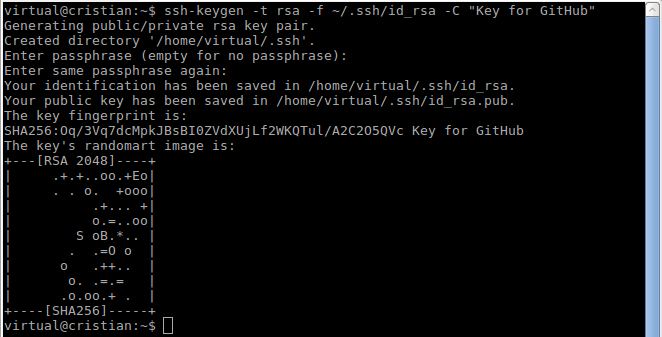
\includegraphics[scale = 0.9]{img/ssh_key.png}
		\caption{Generarea ssh-key}%
		\label{fig:generarea_ssh_key}
	\end{center}


	\begin{center}
		\centering
		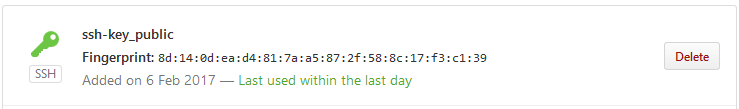
\includegraphics[scale = 0.8]{img/add_key_onserver.png}
		\caption{Adaugarea ssh-key pe server}%
		\label{fig:add_key_onserver}
	\end{center}

	\begin{center}
		\centering
		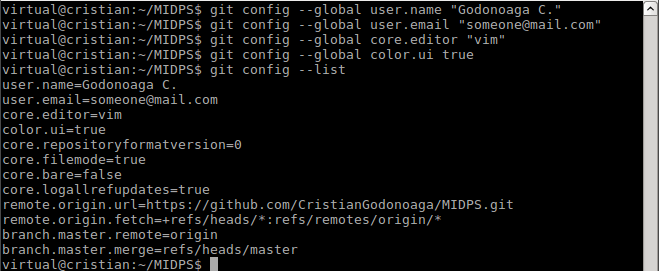
\includegraphics[scale = 0.9]{img/git_config.png}
		\caption{Configurare VCS}%
		\label{fig:git_config}
	\end{center}
\end{figure}
\clearpage